\section{Cache-Speicher}

\textbf{Hintergrund}
\begin{items}
	\item Lücke zwischen Verarbeitungs- (CPU) und Zugriffsgeschwindigkeit (DRAM) immer größer
	\item \underline{Lösung}: Hierarchische Anordnung verschiedener Speicher \\*
		\( \leadsto \) Ausgleich der unterschiedlichen Zugriffszeiten
	\item \underline{Strategien}:
	\begin{enumeration}
		\item \textbf{Cache-Speicher}: Kurze Zugriffszeiten \\*
			\( \leadsto \) Beschleunigung Prozessorzugriff
		\item \textbf{Virtueller Speicher}: Vergrößerung des tatsählich vorhandenen Hauptspeichers (z.B. bei gleichzeitiger Bearbeitung mehrerer Prozesse)
	\end{enumeration}
	\item Leistung abhängig von Eigenschaften der Speichertechnologien, Adressierung und Organisation
\end{items}
\begin{figure}[H]\centering\label{Speicherhierarchie}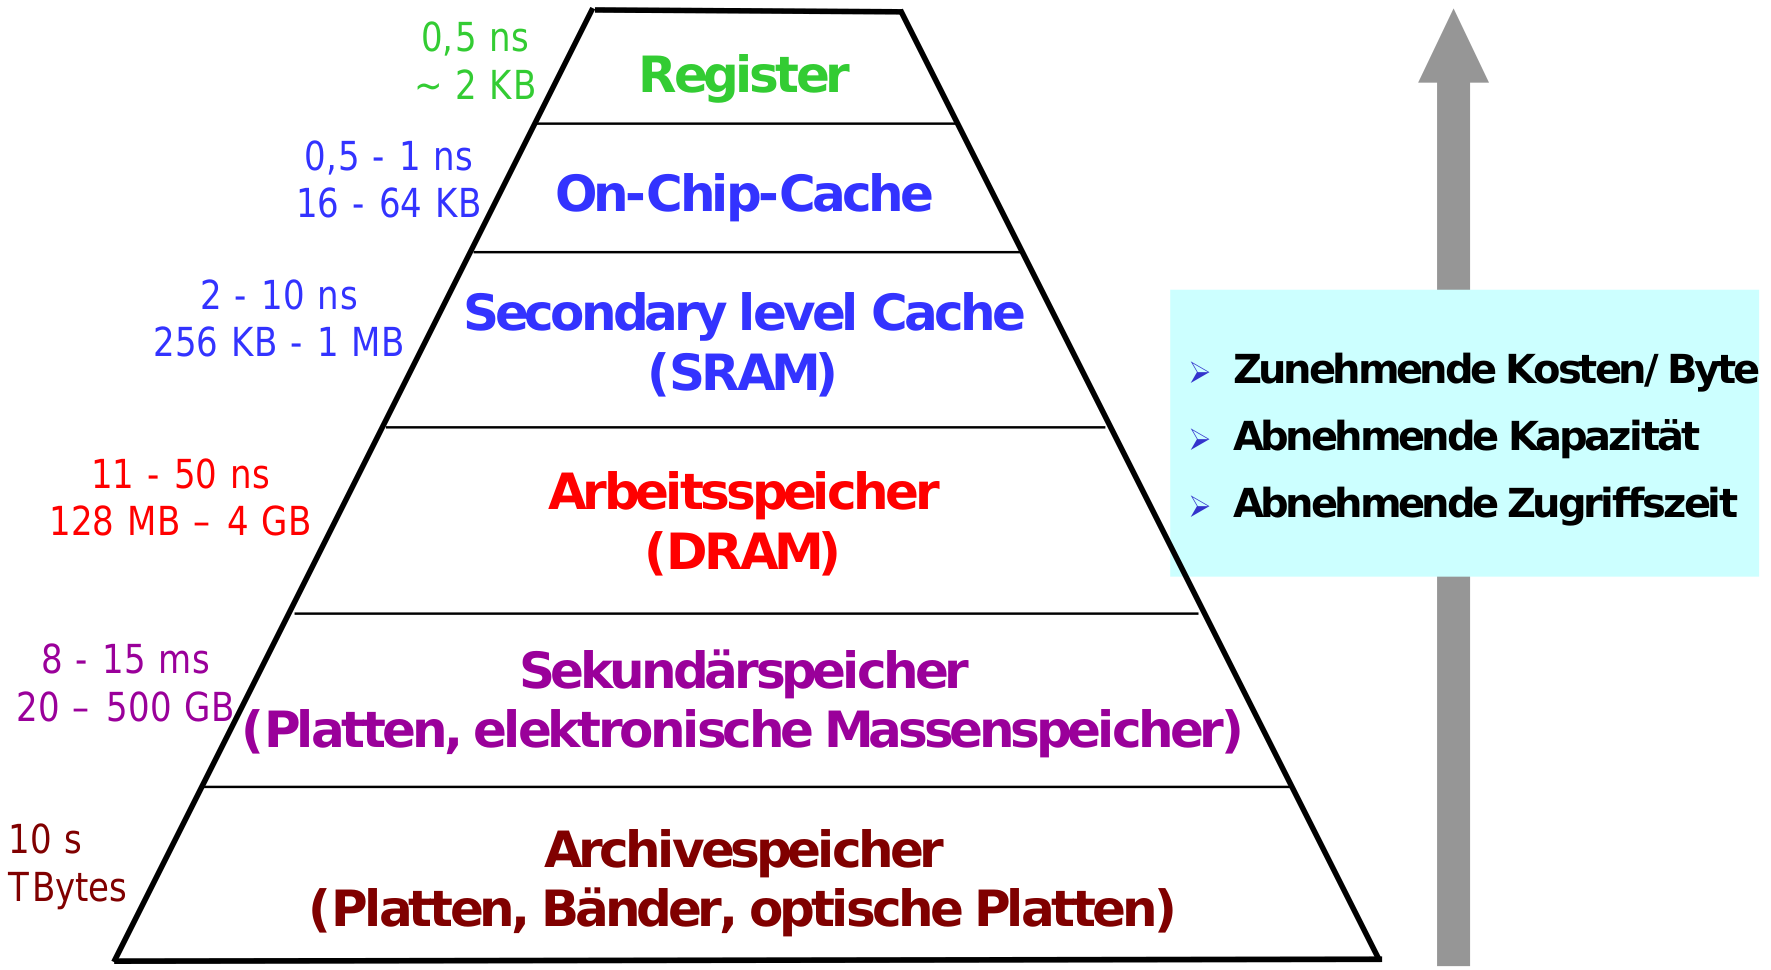
\includegraphics[width=0.33\textwidth]{Speicherhierarchie}\end{figure}

\textbf{CPU-Cache}
\begin{items}
	\item kleiner, schneller Pufferspeicher
	\item speichert \emph{Kopien} von Hauptspeicherteilen, auf die mit hoher Wahrscheinlichkeit als nächstes zugegriffen wird
	\item Effizienz durch \emph{Lokalitätseigenschaft} von Programmen:
	\begin{enumeration}
		\item \textbf{zeitliche Lokalität}: zukünftig angesprochene Information mit hoher Wahrscheinlichkeit schon einmal angesprochen worden (z.B. Schleifen)
		\item \textbf{örtliche Lokalität}: zukünftig angesprochene Information mit hoher Wahrscheinlichkeit in Nähe des bisherigen Zugriffs (z.B. Arrays)
	\end{enumeration}
	\item \emph{Cache-Controller} lädt alle Daten in Cache, auf die Prozessor zugreift
	\item Daten werden aus Cache verdrängt, wenn sie nicht mehr benötigt werden
\end{items}

\textbf{Cache -- Funktionsweise}
\begin{items}
	\item \underline{Lesezugriff}: \( \mu \)P überprüft davor ob Datum in Cache steht \\*
		- \textbf{read hit}: Datum wird ohne Wartezyklen aus Cache geladen \\*
		- \textbf{read miss}: Datum wird mit Wartezyklen aus Arbeitsspeicher \\* \phantom{-} geladen und in Cache eingefügt
	\item \underline{Schreibzugriff}: \\*
		- \textbf{write miss}: Datum wird in DRAM und Cache geschrieben \\*
		- \textbf{write hit}: verschiedene Verfahren möglich
\end{items}

\textbf{Schreibzugriff -- Durchschreibverfahren}
\begin{items}
	\item Datum wird von CPU immer gleichzeitig in Cache- und Arbeitsspeicher geschrieben
	\item \underline{Vorteil}: Konsistenzgarantie zwischen Cache und DRAM
	\item \underline{Nachteil}: Schreibzugriffe benötigen immer langsame Zykluszeit von Hauptspeicher, belasten Systembus
\end{items}

\textbf{Schreibzugriff -- gepuffertes Durchschreibverfahren}
\begin{items}
	\item Verwendung von \emph{Schreib-Puffer}, der zu schreibende Daten temporär aufnimmt
	\item Daten werden dann automatisch von Cache-Controller in Hauptspeicher übertragen
\end{items}

\textbf{Schreibzugriff -- Rückschreibverfahren}
\begin{items}
	\item Datum wird von CPU nur in Cachespeicher geschrieben und durch spezielles Bit (\emph{dirty bit}) gekennzeichnet
	\item Arbeitsspeicher wird nur geändert, wenn \emph{dirty}-Datum aus Cache verdrängt wird
	\item \underline{Vorteil}: Alle Schreibzugriffe mit schneller Cache-Zykluszeit abwickelbar
	\item \underline{Nachteil}: Konsistenzprobleme zwischen Cache- und Hauptspeicher
\end{items}

\textbf{Konsistenzprobleme}
\begin{items}
	\item Andere Systemkomponenten (z.B. DMA-Controller) finden ggf "`veraltete Daten"' in DRAM vor, die von CPU längst geändert wurden
	\item Andere Systemkomponenten können Daten in Hauptspeicher ändern, während CPU noch mit alten Daten aus Cache arbeitet
	\item \( \leadsto \) aufwendige Verfahren bei Cache-Steuerung zur Inkonsistenzvermeidung erforderlich
\end{items}

\textbf{Begriffe}
\begin{items}
	\item \underline{Hit-Rate}: = Anzahl Treffer pro Anzahl Zugriffe
	\item \underline{Mittlere Zugriffszeit}: \\*
		\( t_{\text{access}} = (\text{Hit-Rate})t_\text{hit}+(1-\text{Hit-Rate})t_\text{miss} \)
\end{items}

\textbf{Cache-Speicher -- Aufbau}
\begin{items}
	\item Besteht aus drei Teilen:
	\begin{enumeration}
		\item \textbf{Datenspeicher}: im Cache abgelegte Daten
		\item \textbf{Adressspeicher}: Adresse dieses Datums im RAM
		\item \textbf{Statusbits}: Geben an, ob Informationen gültig sind
	\end{enumeration}
	\item Zusammen: \emph{cache-line}
	\item \underline{Komparator}: ermittelt, ob zu Adressbus gehörendes Datum in Cache abgelegt ist
\end{items}